\section{Лекция номер 7}

\subsection{Функциональные последовательности}

\begin{conj}
    Поточечная сходимость.

    $f_n, f: E \to \R$

    $f_n \to f$ поточечно ($f_n$ пототечно сходится к $f$), если

    $$
        \forall x \in E \; \lim_{n \to +\infty} f_n(x) = f(x)
    $$
\end{conj}

\begin{conj}
    Равномерная сходимость.

    $f_n, f: E \to \R$

    $f_n \doublerightarrow f$ на $E$ ($f_n$ равномерно сходится к $f$ на $E$), если

    $$
        \forall \; \varepsilon > 0 \; \exists N: \; \forall n \geqslant N \; \forall x \in E \; \abs{f_n(x) - f(x)} < \varepsilon
    $$
\end{conj}

\notice 
\begin{enumerate}
    \item Поточечная сходимость с кванторами:
    $$
        \forall x \in E \; \forall \varepsilon > 0 \; \exists N: \forall n \geqslant N \; \abs{f_n(x) - f(x)} < \varepsilon
    $$
    \item $f_n \doublerightarrow f \Longrightarrow f_n \to f$
\end{enumerate}

\begin{example}
    $E = (0, 1), \, f_n(x) = x^n, \, f_n \to f \equiv 0$

Поймём, что равномерной сходимости нет:

$\forall \varepsilon > 0 \; \exists N: \; \forall n \geqslant N \; \forall x \in (0, 1): \; x^n < \varepsilon \Longrightarrow 1 = \lim_{x \to 1^{-}} x^n \leqslant \varepsilon$ (т.е. для $\varepsilon < 1$ это неверно)
\end{example}

\vspace*{7mm}

\textbf{Поясняющая картинка к равномерной сходимости}.

Пусть $f_n \rightrightarrows f$. 
Тогда условие \[ \forall \; \varepsilon > 0 \; \exists N: \; \forall n \geqslant N \; \forall x \in E \; \abs{f_n(x) - f(x)} < \varepsilon \] 
означает, что для любого $\varepsilon > 0$ найдется такой достаточно большой номер $N$, что, начиная с него, графики всех функций $f_n(x)$ будут лежать в полоске шириной $2\varepsilon$ относительно графика $f(x)$:
\begin{center}
    %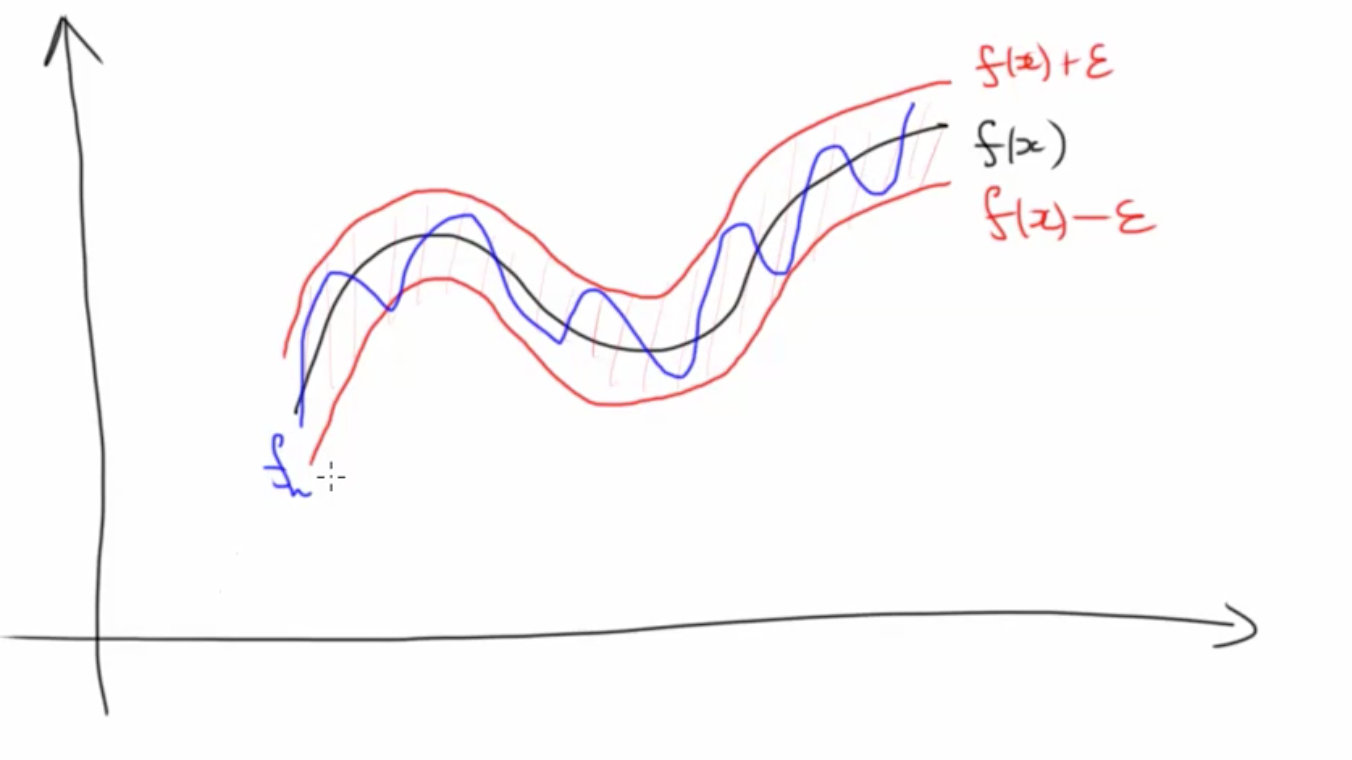
\includegraphics[scale=0.5]{Uniform_convergence.png} 
    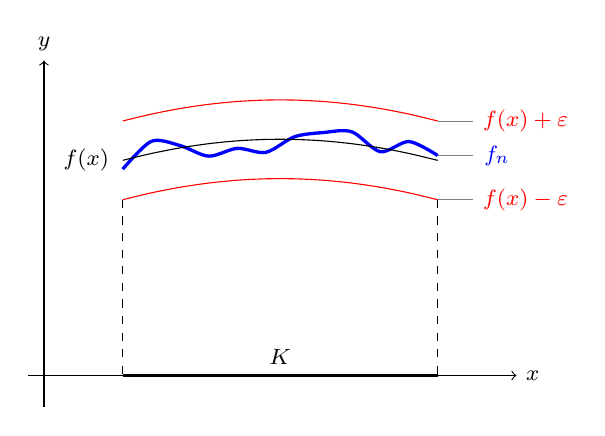
\begin{tikzpicture}[auto,
        B/.style = {decorate,
                    decoration={brace, amplitude=3pt,
                    pre=moveto,pre length=1pt,post=moveto,post length=1pt,
                    raise=1mm}},
           domain = -30:30, samples=12, smooth,
             font = \footnotesize
                                ]
        % coordinates
        \draw[->] (-0.2,0) -- (6,0) node[right]{$x$};
        \draw[->] (0,-0.4) -- (0,4) node[above]{$y$};
        % curve
        \draw[very thick, blue] 
            plot ({(45+\x)/15},{1+rand/5+2*cos(\x)})
            node[coordinate,pin=0:$f_n$] {};
        % convergence borders
        \draw[red]  plot ({(45+\x)/15},{1.5+2*cos(\x)}) 
                    node[coordinate,pin=0:$f(x)+\varepsilon$] {};
        \draw[black] plot ({(45+\x)/15},{1.0+2*cos(\x)}) coordinate (e2);
        \draw[red]  plot ({(45+\x)/15},{0.5+2*cos(\x)}) 
                    node[coordinate,pin=0:$f(x)-\varepsilon$] {};
    
        % labels on the left side
        \draw (1,{1.75+cos(-10)}) node[left=0.5mm]   {$f(x)$} ++ (0,1);
        \draw[dashed]   (1,{0.5+2*cos(30)}) -- (1,0)
                        (5,{0.5+2*cos(30)}) -- (5,0);
    
        \draw[very thick]    (1,0) -- node[above] {$K$} (5,0);
        
    \end{tikzpicture}   
\end{center}

\vspace*{7mm}

\begin{conj}
    Равномерно ограниченная последовательность.

    $f_n: E \to \R$~--- равномерно ограниченная последовательность, если

    $$
        \exists \; M: \; \forall x \in E, \; \forall n \in \N: \; |f_n(x)| \geqslant M 
    $$
\end{conj}

\begin{theorem}
    $f_n \doublerightarrow f$ на $E \Longleftrightarrow \sup_{x \in E}{\abs{f_n(x) - f(x)}} \to 0$

    \begin{proof}
        "$\Longrightarrow:$"

        $f_n \doublerightarrow f$ на $E \Longleftrightarrow \forall \varepsilon > 0 \; \exists N \; \forall n \geqslant N \; \forall x \in E: \abs{f_n(x) - f(x)} < \varepsilon$ 

        $\Longrightarrow \varepsilon$~--- верхняя граница для $\abs{f_n(x) - f(x)} \Longrightarrow \sup_{x \in E}{\abs{f_n(x) - f(x)}} \leqslant \varepsilon$ 

        $\Longrightarrow \forall \varepsilon > 0 \; \exists N: \; \forall n \geqslant N \; \sup_{x \in E}{\abs{f_n(x) - f(x)}} \leqslant \varepsilon$ 

        $\Longleftrightarrow \sup_{x \in E}{\abs{f_n(x) - f(x)}} \to 0$

        "$\Longleftarrow:$"

        $\sup_{x \in E}{\abs{f_n(x) - f(x)}} \to 0 \Longleftrightarrow \forall \varepsilon > 0 \; \exists N: \; \forall n \geqslant N \; \sup_{x \in E}{\abs{f_n(x) - f(x)}} < \varepsilon$ 

        т.к. $\abs{f_n(x) - f(x)} \leqslant \sup_{x \in E}{\abs{f_n(x) - f(x)}}$, то 

        $\forall \varepsilon > 0 \; \exists N: \forall n \geqslant N \; \abs{f_n(x) - f(x)} < \varepsilon$
    \end{proof}

\end{theorem}

\follow

\begin{enumerate}
    \item $\abs{f_n(x) - f(x)} \leqslant a_n \; \forall x \in E$ и $a_n \to 0$, то $f_n \doublerightarrow f$ на $E$
    \begin{proof}
        $\abs{f_n(x) - f(x)} \leqslant a_n \Longrightarrow \sup_{x \in E}{\abs{f_n(x) - f(x)}} \leqslant a_n \to 0$
    \end{proof}
    \item $f_n \not \doublerightarrow f$ на $E$ $\Longleftrightarrow \exists x_n \in E$, т.ч. $f_n(x_n) - f(x_n) \not \to 0$
    \begin{proof}
        "$\Longleftarrow:$"
         
        $\sup_{x \in E}{\abs{f_n(x) - f(x)}} \geqslant \abs{f_n(x) - f(x)} \not \to 0 \Longrightarrow \sup_{x \in E}{\abs{f_n(x) - f(x)}} \not \to 0$

        "$\Longrightarrow:$"

        $f_n \not \doublerightarrow f \Longrightarrow \sup_{x \in E}{\abs{f_n(x) - f(x)}} \not \to 0 \Longrightarrow$ легко можно выбрать такую $x_n$, что $f_n(x_n) - f(x_n) \not \to 0$
    \end{proof}
\end{enumerate}

\begin{example}
    $f_n(x) = x^n$

    $\sup_{x \in (0, 1)}{x^n} = 1 \not \to 0$
\end{example}


\begin{theorem}

    Если $f_n$ равномерно ограничена, $g_n \doublerightarrow 0$

    Тогда $f_n \cdot g_n \doublerightarrow 0$

    \begin{proof}
        $\forall n, \; \forall x \; \abs{f_n(x)} \leqslant M$

        Надо доказать, что $\sup_{x \in E}{\abs{f_n(x) - f(x)}} \to 0$

        $$
            \abs{f_n(x) \cdot g_n(x)} \leqslant M \cdot \abs{g_n(x)} \Longrightarrow \sup_{x \in E}{\abs{f_n(x) - f(x)}} \leqslant M \cdot \sup{\abs{g_n(x)}} \to 0
        $$
    \end{proof}
    
\end{theorem}

\begin{theorem}[Критерий Коши]
    $ $ \\
    $f_n: E \to \R$

    $f_n$~--- равномерно сходится $\Longleftrightarrow \forall \varepsilon > 0 \; \exists N \; \forall n,m \geqslant N: \; \forall x \in E \; \abs{f_n(x) - f_m(x)} < \varepsilon$

    \begin{proof}
        $ $

        "$\Longrightarrow:$"

        $f_n \doublerightarrow f \Longrightarrow \exists N \; \forall n,m \geqslant N: \; \forall x \in E:$

        $\begin{cases}
            \abs{f_n(x) - f(x)} < \frac{\varepsilon}{2} \\
            \abs{f_m(x) - f(x)} < \frac{\varepsilon}{2} 
        \end{cases} \Longrightarrow$
        $\abs{f_n(x) - f_m(x)} \leqslant \abs{f_n(x) - f(x)} + \abs{f(x) - f_m(x)} < \varepsilon$

        $\Longrightarrow \abs{f_n(x) - f_m(x)} < \varepsilon \Longrightarrow f_n$ удовлетворяет условию.
        
        "$\Longleftarrow:$"

        Зафиксируем $x:$

        $\forall \varepsilon > 0 \; \exists N: \; \forall n, m \geqslant N \; \abs{f_n(x) - f_m(x)} < \varepsilon$

        $\Longrightarrow f_n(x)$~--- фундаментальная последовательность $\Longrightarrow \exists$ конечный $\lim\limits_{n \to +\infty} f_n(x) =: f(x)$

        $\forall \varepsilon > 0 \; \exists N: \; \forall n, m \geqslant N \; \forall x \in E \; \abs{f_n(x) - f_m(x)} < \varepsilon$
        $\stackrel{m \to +\infty}{\Longrightarrow} \abs{f_n(x) - f(x)} \leqslant \varepsilon \Longrightarrow f_n \doublerightarrow f$ на $E$.

    \end{proof}
\end{theorem}

\begin{conj} Нормированое пространство ограниченных функций

    $l^{\infty}(E) := \{ f: E \to R; f$~--- ограниченая функция \}
    
    $\norm{f}_{l^{\infty}(E)} := \norm{f}_{\infty} := \sup_{x \in E}{\abs{f(x)}}$ (он конечен, т.к. $f$~--- ограничена)

    Аксиомы нормы очевидны (кроме неравенства $\triangle$)

    $\norm{f + g}_{\infty} \leqslant \norm{f}_{\infty} + \norm{g}_{\infty}$
    
    $\sup_{x \in E}{\abs{f(x) + g(x)}} \leqslant \sup_{x \in E}(\abs{f(x)} - \abs{g(x)}) \leqslant \sup_{x \in E}{\abs{f(x)}} + \sup_{x \in E}{\abs{g(x)}} = \norm{f}_{\infty} + \norm{g}_{\infty}$
\end{conj}

\notice 

\begin{enumerate}
    \item $f_n \doublerightarrow f$ на $E$ $\Longleftrightarrow \norm{f_n - f}_{l^{\infty}(E)} \to 0$
    (у нас уже есть такое свойство, здесь просто по определению $\norm{f_n - f}_{l^{\infty}(E)} = \sup_{x \in E}{\abs{f_n(x) - f(x)}}$)
    \item Равномерная сходимость $\Longrightarrow$ сходимость по норме $\norm{\cdot}_{l^{\infty}(E)}$
\end{enumerate}

\begin{theorem}[О полноте нормированного пространства ограниченных функций]
    $ $ 

    $l^{\infty}(E)$~--- полное пространство 

    \begin{proof}
        Нужно доказать, что любая фундоментальная последовательность имеет предел, лежащий в этом пространстве.

        Пусть $f_n$~--- фундоментальная последовательность:

        $$
            \forall \varepsilon > 0 \; \exists N: \; \forall n,m \geqslant N \; \norm{f_n(x) - f_m(x)} < \varepsilon \Longleftrightarrow \sup_{x \in E}{\abs{f_n(x) - f(x)}} < \varepsilon
        $$

        $\Longrightarrow \forall \varepsilon > 0 \; \exists N: \; \forall n,m \geqslant N \; \forall x \in E \; \abs{f_n(x) - f_m(x)} < \varepsilon$~--- критерий Коши $\Longrightarrow f_n \doublerightarrow f$ на $E \Longrightarrow \norm{f_n - f} \to 0$

        Осталось убедиться, что $f$, к которой сходится наша фундоментальная последовательность лежит в нашем пространстве, т.е. является ограниченной функцией:

        Возьмём $\varepsilon = 1: \; \exists N \; \forall n \geqslant N \; \norm{f_n - f} < 1 \Longleftrightarrow \sup_{x \in E}{\abs{f_n(x) - f(x)}} < 1 \Longleftrightarrow \forall x \in E \; \abs{f_{N}(x) - f(x)} < 1 \Longleftrightarrow \abs{f(x)} < 1 + \abs{f_{N}(x)} \leqslant 1 + C$
    \end{proof}

\end{theorem}

\begin{example}
    $f_n(x) = x^n : [0, 1] \to \R$

$f(x) = \begin{cases}
    1 \; if \; x = 1 \\
    0 \; else 
\end{cases}$

$f_n(x) \to f(x)$, где $f(x)$ не является непрерывной (а хотелось бы :(( )

\end{example}

\begin{theorem}
    $f_n: E \to \R$ непрерына в $(\cdot) a \in E$ и $f_n \doublerightarrow f$ на $E$

    Тогда $f$ непрерывна в $(\cdot) a$

    \begin{proof}
        Зафиксируем $\varepsilon > 0$

        $\exists N \; \forall n \geqslant N: \; \forall x \in E \; \abs{f_n(x) - f(x)} < \varepsilon$

        Зафиксируем $n_0 > N$, тогда $\forall x \in E \; \abs{f_{n_0}(x) - f(x)} < \varepsilon$

        Далее,  $\forall x \in E: \; \abs{f(x) - f(a)} \leqslant \underbrace{\abs{f(x) - f_{n_0}(x)}}_{\text{$< \varepsilon$}} + \abs{f_n(x) - f_n(a)} + \underbrace{\abs{f_n(a) - f(a)}}_{\text{$< \varepsilon$}} < 2 \cdot \varepsilon + \abs{f_n(x) - f_n(a)}$

        т.к. $f_n$~--- непрерывная в $(\cdot) a$, то:

        $\exists \delta > 0: \; \forall x \in E: \; \abs{x - a} < \delta: \; \abs{f_n(x) - f(a)} < \varepsilon$ \\
        Возьмём эту $\delta:$ тогда $\abs{f_n(x) - f_n(a)} < \varepsilon$ и тогда $\abs{f(x) - f(a)} < 3 \cdot \varepsilon$

        Т.е. мы взяли $\varepsilon$, смогли подобрать $\delta > \abs{x - a}$ и получили, что $\abs{f(x) - f(a)} < 3 \cdot \varepsilon$, т.е. $f(x)$~--- ограничена в $(\cdot) a$.
    \end{proof}
\end{theorem}

\follow (т. Стокса-Зайделя)

Если $f_n \in C(E)$~--- непрерывны на $E$ и $f_n \doublerightarrow f$ на $E$, то $f \in C(E)$

\begin{conj}
    Нормированное пространство непрерывных функций.

    Пространство $C(K)$, $K$~--- компакт.

    $C(K) := \{ f: K \to \R; f$~--- непрерывна $\} \subset l^{\infty}(K)$ (т.к. функция, непрерывная на компакте, ограничена всегда)

    $\norm{f}_{C(K)} := \max_{x \in K}{\abs{f(x)}} = \sup_{x \in K}{\abs{f(x)}}$ (для непрерывной на компакте функции максимум где-то достигается)

    $C(K)$~--- линейное подпространство $l^{\infty}(K)$
    $f + g \in C(K), \; c \cdot f \in C(K)$
\end{conj}

\follow 

$C(K)$~--- замкнутое подпространство $l^{\infty}(K)$

\begin{proof}
    Берём $f_n \in C(K)$ и $\norm{f_n - f} \to 0 \Longleftrightarrow f_n \doublerightarrow f$ на $K \Longleftrightarrow f$~--- непрерывна.
\end{proof}

\begin{theorem}
    Замкнутное подпространство полного пространства~--- полное пространство.

    \begin{proof}
        Пусть $X$~--- полное пространство, а $Y$~--- подпространство в $X$.

        Возьмём фундоментальную последовательность в $Y: a_n \in Y \Longrightarrow a_n$~--- фундоментальна в $X$

        $X$~--- полное $\Longrightarrow a_n \to a \in X$

        Но т.к. $Y$~--- замкнутое, то $a \in Y \Longrightarrow Y$~--- полное (т.к. $\lim a_n = a \in Y$)
    \end{proof}
\end{theorem}

\follow \; $C(K)$~--- полное нормированное пространство.

\subsection{Функциональные ряды}
%after breakout 